%% abtex2-modelo-slides.tex, v-1.0 gfabinhomat
%% Copyright 2012-2016 by abnTeX2 group at http://www.abntex.net.br/ 
%%
%% This work may be distributed and/or modified under the
%% conditions of the LaTeX Project Public License, either version 1.3
%% of this license or (at your option) any later version.
%% The latest version of this license is in
%%   http://www.latex-project.org/lppl.txt
%% and version 1.3 or later is part of all distributions of LaTeX
%% version 2005/12/01 or later.
%%
%% This work has the LPPL maintenance status `maintained'.
%% 
%% The Current Maintainer of this work is Fábio Rodrigues Silva, 
%% member of abnTeX2 team, led by Lauro César Araujo. 
%% Further information are available on 
%% http://www.abntex.net.br/
%%
%% This work consists of the files abntex2-modelo-slides.tex, 
%% abntex2-modelo-references.bib and abntex2-modelo-marca.pdf
%%
%% Modelo desenvolvido por Fábio Rodrigues Silva (gfabinhomat@gmail.com)
%% Mais informações podem ser obtidas no guia do usuário Beamer 
%% (http://linorg.usp.br/CTAN/macros/latex/contrib/beamer/doc/beameruserguide.pdf)
%% Informações rápidas podem ser acessadas em http://en.wikibooks.org/wiki/LaTeX/Presentations


% Apresentações em widescreen. Outros valores possíveis: 1610, 149, 54, 43 e 32.
% Por padrão, as apresentações são no formato 4:3 (sem o aspectratio).
%\documentclass[aspectratio=169]{beamer}	 	
\documentclass[]{beamer}	 	

\usetheme{Berlin}
\usecolortheme{default}
\usefonttheme[onlymath]{serif}			% para fontes matemáticas
% Enconte mais temas e cores em http://www.hartwork.org/beamer-theme-matrix/ 
% Veja também http://deic.uab.es/~iblanes/beamer_gallery/index.html

% Customizações de Cores: fg significa cor do texto e bg é cor do fundo
\setbeamercolor{normal text}{fg=black}
\setbeamercolor{alerted text}{fg=red}
\setbeamercolor{author}{fg=blue}
\setbeamercolor{institute}{fg=blue}
\setbeamercolor{date}{fg=green}
\setbeamercolor{frametitle}{fg=white}
\setbeamercolor{framesubtitle}{fg=white}
\setbeamercolor{block title}{bg=blue, fg=white}		%Cor do título
\setbeamercolor{block body}{bg=gray, fg=darkgray}	%Cor do texto (bg= fundo; fg=texto)
\setbeamerfont{title}{family=\rmfamily,series=\bfseries,size={\fontsize{14}{16}}}
%\setbeamertemplate{caption}[numbered]
%\setbeamertemplate{bibliography item}{[\theenumiv]}
\setbeamertemplate{bibliography item}{}

% ---
% PACOTES
% ---
\usepackage[alf]{abntex2cite}		% Citações padrão ABNT
\usepackage[brazil]{babel}		% Idioma do documento
\usepackage{color}			% Controle das cores
\usepackage[T1]{fontenc}		% Selecao de codigos de fonte.
\usepackage{graphicx}			% Inclusão de gráficos
\usepackage[utf8]{inputenc}		% Codificacao do documento (conversão automática dos acentos)
\usepackage{txfonts}			% Fontes virtuais
\usepackage{subfig}
\usepackage{sidecap}
\usepackage{verbatim}
\graphicspath{{imagens/}}




\usepackage{lmodern}			% Usa a fonte Latin Modern			
\usepackage[utf8]{inputenc}		% Codificacao do documento (conversão automática dos acentos)
\usepackage{lastpage}			% Usado pela Ficha catalográfica
\usepackage{indentfirst}		% Indenta o primeiro parágrafo de cada seção.



\usepackage{subfig}
\usepackage{graphicx}			% Inclusão de gráficos

\usepackage{microtype} 			% para melhorias de justificação
\usepackage{soul}
\usepackage{amssymb}
\usepackage{amsmath}
\usepackage{spreadtab}
\usepackage{multirow}
\usepackage{amsthm}
\usepackage{url}


\usepackage[portuguese, ruled, linesnumbered]{algorithm2e}

\usepackage{algorithmic}

% Utilizado para customizar as fontes das equações 
\usepackage{fixmath}
\usepackage{verbatim}

%\usepackage[brazilian,hyperpageref]{backref}	 % Paginas com as citações na bibl


\graphicspath{{imagens/}}


\usepackage{longtable}
%\usepackage{csvsimple,booktabs}
\usepackage{pgfplotstable}
\usepackage{filecontents}
%\usepackage{tabu}
\usepackage{makecell}
\usepackage{booktabs}
\usepackage{float}

\usepackage{multirow}
%\usepackage[table]{xcolor}

%\usepackage{colortbl}
%\definecolor{lightgray}{gray}{0.9}

\usepackage[brazil]{babel} % for European Portuguese use portuguese
\usepackage[fixlanguage]{babelbib}
\selectbiblanguage{brazil}
\citeoption{abnt-etal-cite=2}
% ---


\title{Uma alternativa aos métodos de filtragem de dados de sensores utilizando intervalo de confiança}
\author[Tales Monteiro Melquiades]{Tales Monteiro Melquiades \\ Orientador: Prof. Me. Marco Antonio Firmino De Sousa
{\\ \footnotesize\ttfamily talesmelquiades@hotmail.com}}
\institute{%
	Universidade Estadual do Tocantins - UNITINS
	%\par 
	\\
	Curso de Sistemas de Informação
}
\date{2022}



% --- Informações do documento ---

% ---

% ----------------- INÍCIO DO DOCUMENTO --------------------------------------
\begin{document}

% ----------------- NOVO SLIDE --------------------------------
\begin{frame}

\begin{minipage}{1\linewidth}
  \centering
  \center
  
\includegraphics[width=0.4\textwidth]{/home/tales/git/tcc/imagens/unitins.png}
 
\end{minipage}

\titlepage

\end{frame}

% ----------------- NOVO SLIDE --------------------------------
\begin{frame}{Sumário}
\tableofcontents
\end{frame}

% ----------------- NOVO SLIDE --------------------------------
\section{Introdução}
\begin{frame}{justificativa}
%\framesubtitle{Otimização}
	\begin{itemize}
		\item Sensores;
		\item Ruído;
		\item Filtragem de dados;
		\item Algoritmos de filtragem;
		\item Sistemas embarcados.
	\end{itemize}
\end{frame}

% ----------------- NOVO SLIDE --------------------------------

\begin{frame}{Objetivos}
	\begin{itemize}
		\item Testar o método de intervalo de confiança, como uma alternativa aos métodos tradicionais para obtenção de dados provindos de sensores sem interferência de ruídos.
	\end{itemize}

\end{frame}

\begin{frame}{Objetivos Específicos}

	\begin{itemize}
		\item Realizar uma revisão bibliométrica de trabalhos que utilizam de métodos probabilísticos para filtragem de dados de sensores;
		\item Avaliar a utilização do método aqui proposto como uma alternativa aos métodos de média móvel e média móvel ponderada;
		\item Escrever funções de filtragem utilizando os métodos de Desvio padrão e Intervalo de confiança;
		% \item Demonstrar os resultados objetivos.
	\end{itemize}
	
\end{frame}

% ----------------- NOVO SLIDE --------------------------------

\section{Revisão de literatura}
% \begin{frame}{Conceitos de Otimização}
% 	\framesubtitle{Região de busca e Ponto ótimo}

% 	\begin{figure}[!htb]
% 		\begin{center}
% 			\includegraphics[scale=0.5]{imagens/grafico_ponto_busca}
% 		\end{center}
% 		\label{figura:grafico_ponto_busca}
% 		\caption{Região de busca e Ponto ótimo - (AZUMA, 2011)}	
% 	\end{figure}
	
% \end{frame}

\begin{frame}{Revisão de literatura}
	\framesubtitle{Intervalo de confiança}
	
	\begin{enumerate}
		\item De acordo com (HENRIQUES, 2011) o intervalo de confiança é um dos procedimentos gerais de inferência estatística que pode aplicar-se a diversos campos de problemas;
	\end{enumerate}
		
\end{frame}

\begin{frame}{Revisão de literatura}
	\framesubtitle{Filtragem de dados de sensores}
	
	\begin{enumerate}
		\item Revisão bibliométrica;
		\item IEEE de 2018 a 2022;
		\item redução de ruído; 
		\item algoritmos de filtragem;
		\item sensores;
		\item 450 conferências;
		\item 215 artigos;
		\item 8 artigos com acesso antecipado;
		\item 2 revistas;
	\end{enumerate}
		
\end{frame}

\begin{frame}{Revisão bibliométrica}
	\framesubtitle{Filtragem de dados de sensores}
	
	\begin{figure}[!htb]	
		\begin{center}
			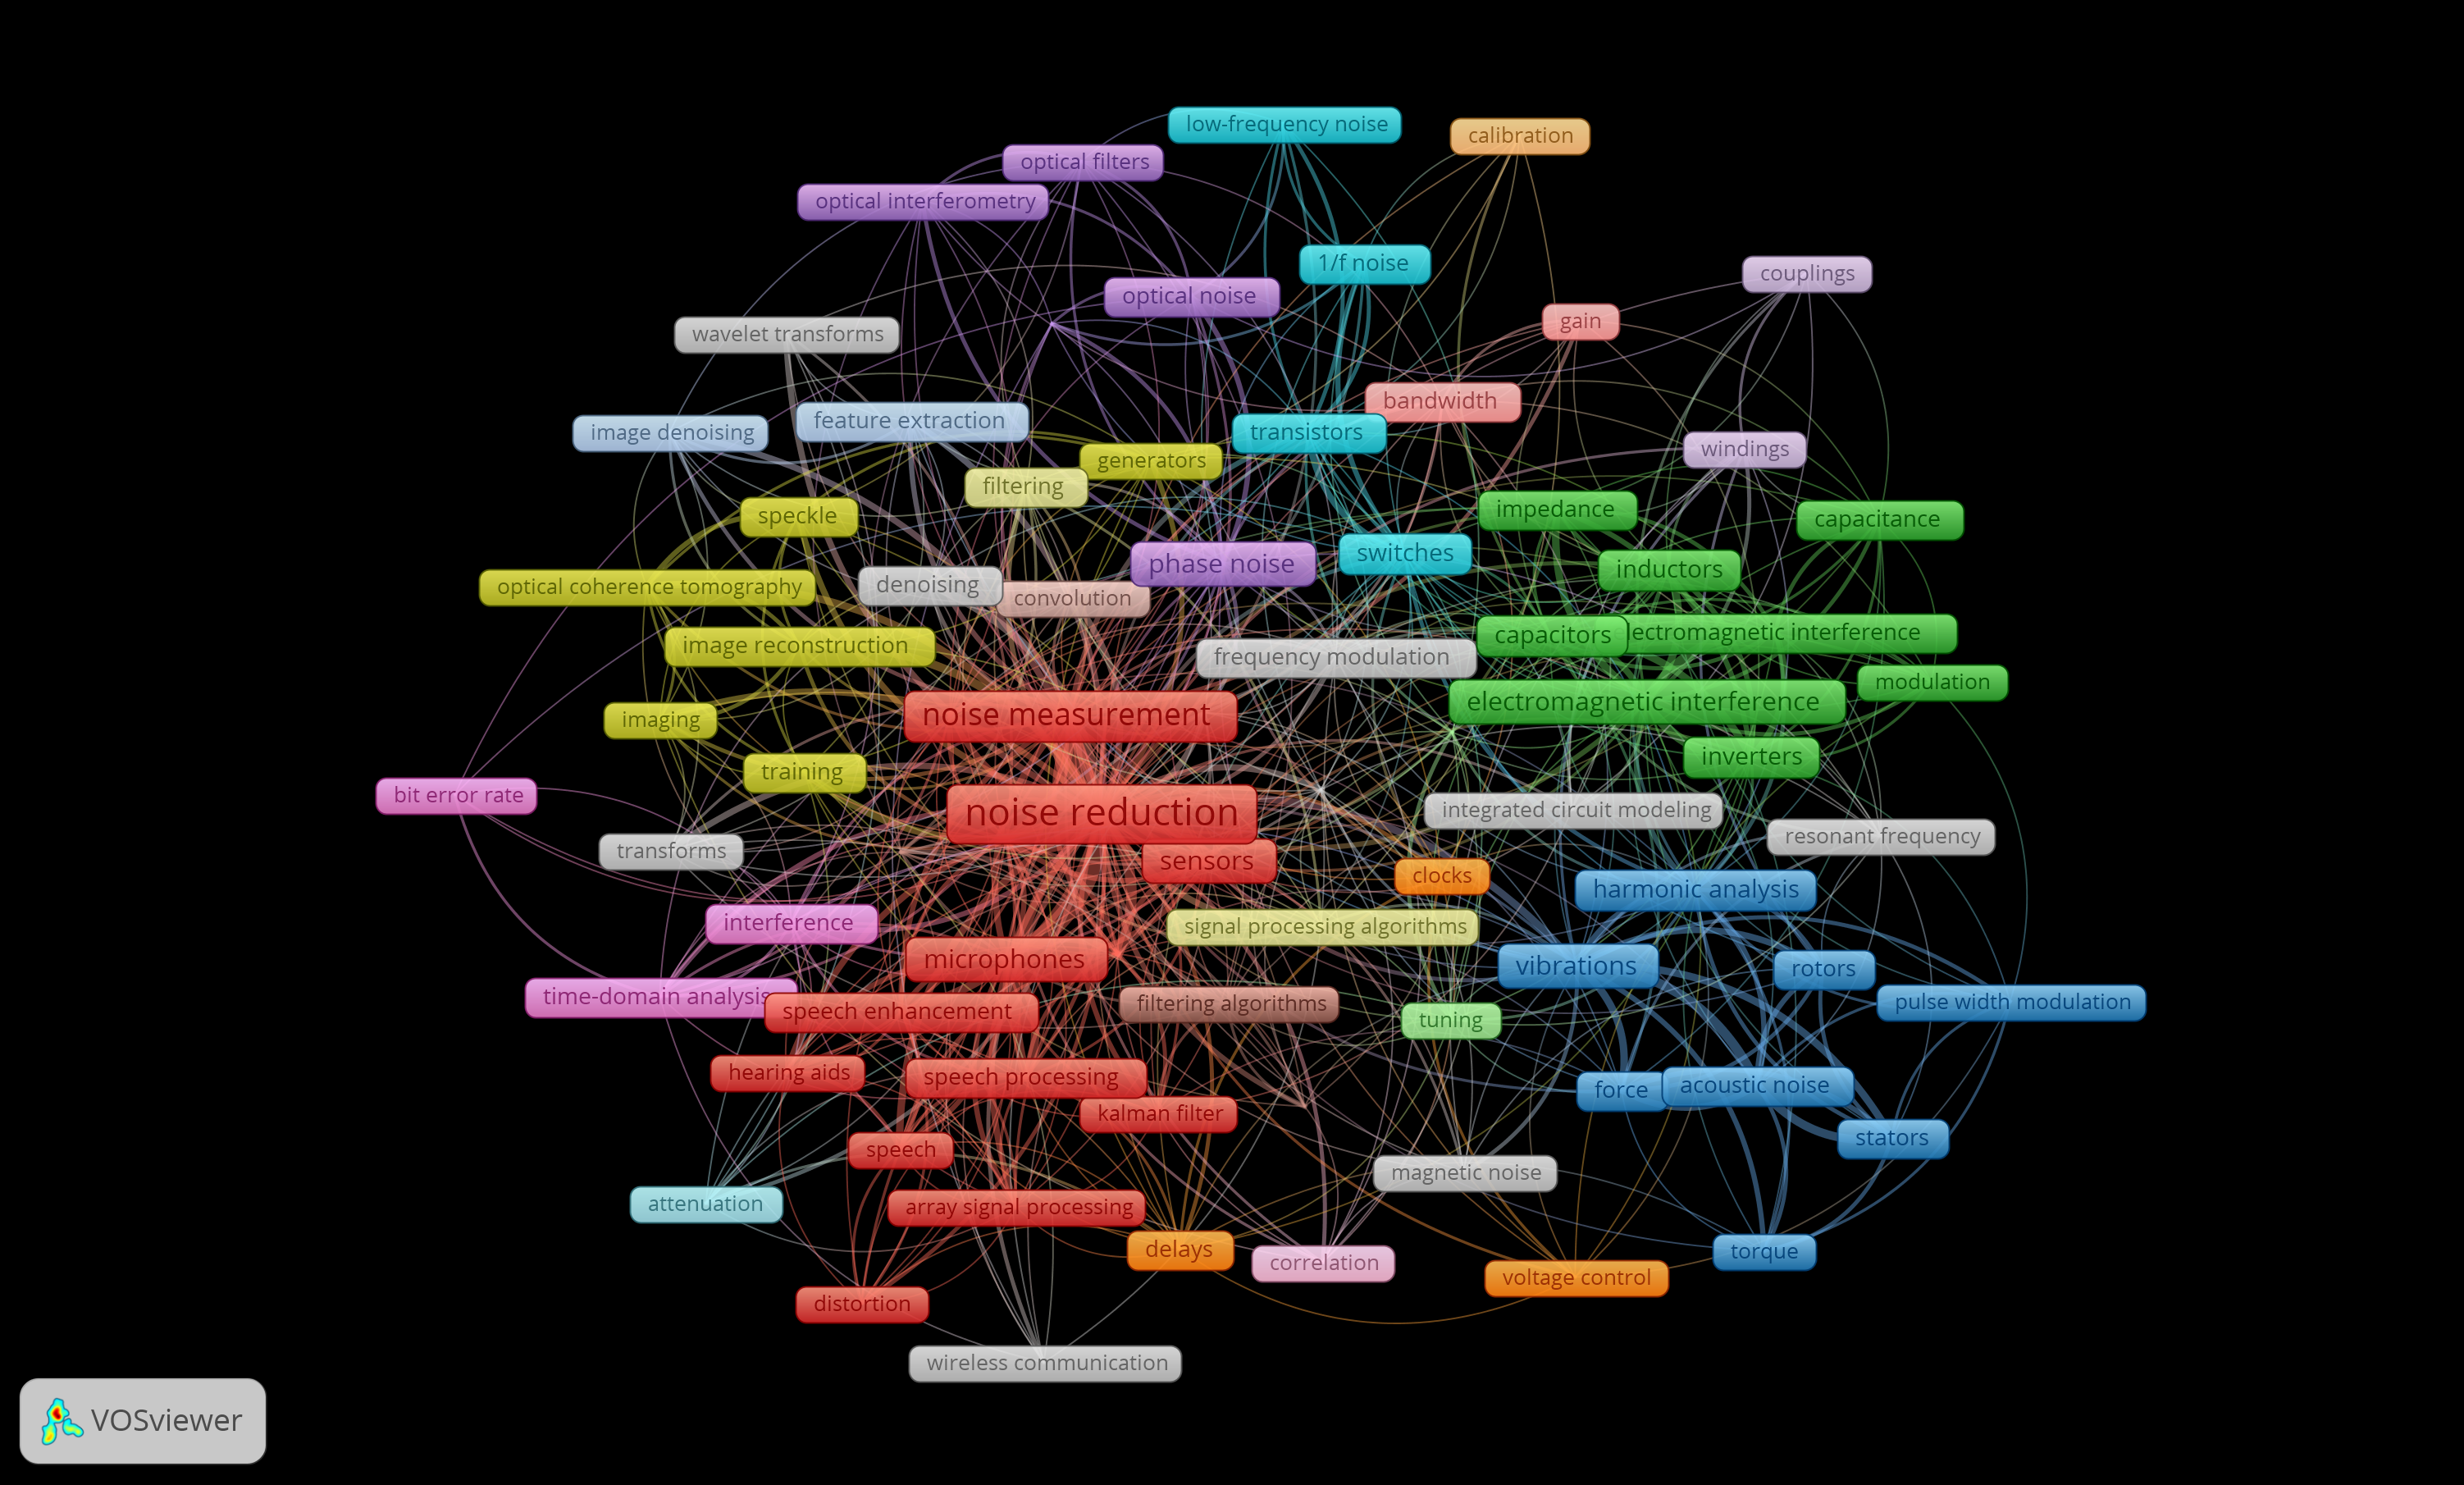
\includegraphics[width=10cm,height=6cm]{../anexos/ris/IEEE/Noise_reduction_and_noise_abatement_andsensor_filtering_algorithm/network_visualization_with_lines.png}
		\end{center}
		\caption{Autor com base no Software VOSViwer}
		\label{figura:network_visualization_with_lines}
	\end{figure}	

\end{frame}

\begin{frame}{Revisão bibliométrica}
	\framesubtitle{Filtragem de dados de sensores}
	
	\begin{figure}[!htb]	
		\begin{center}
			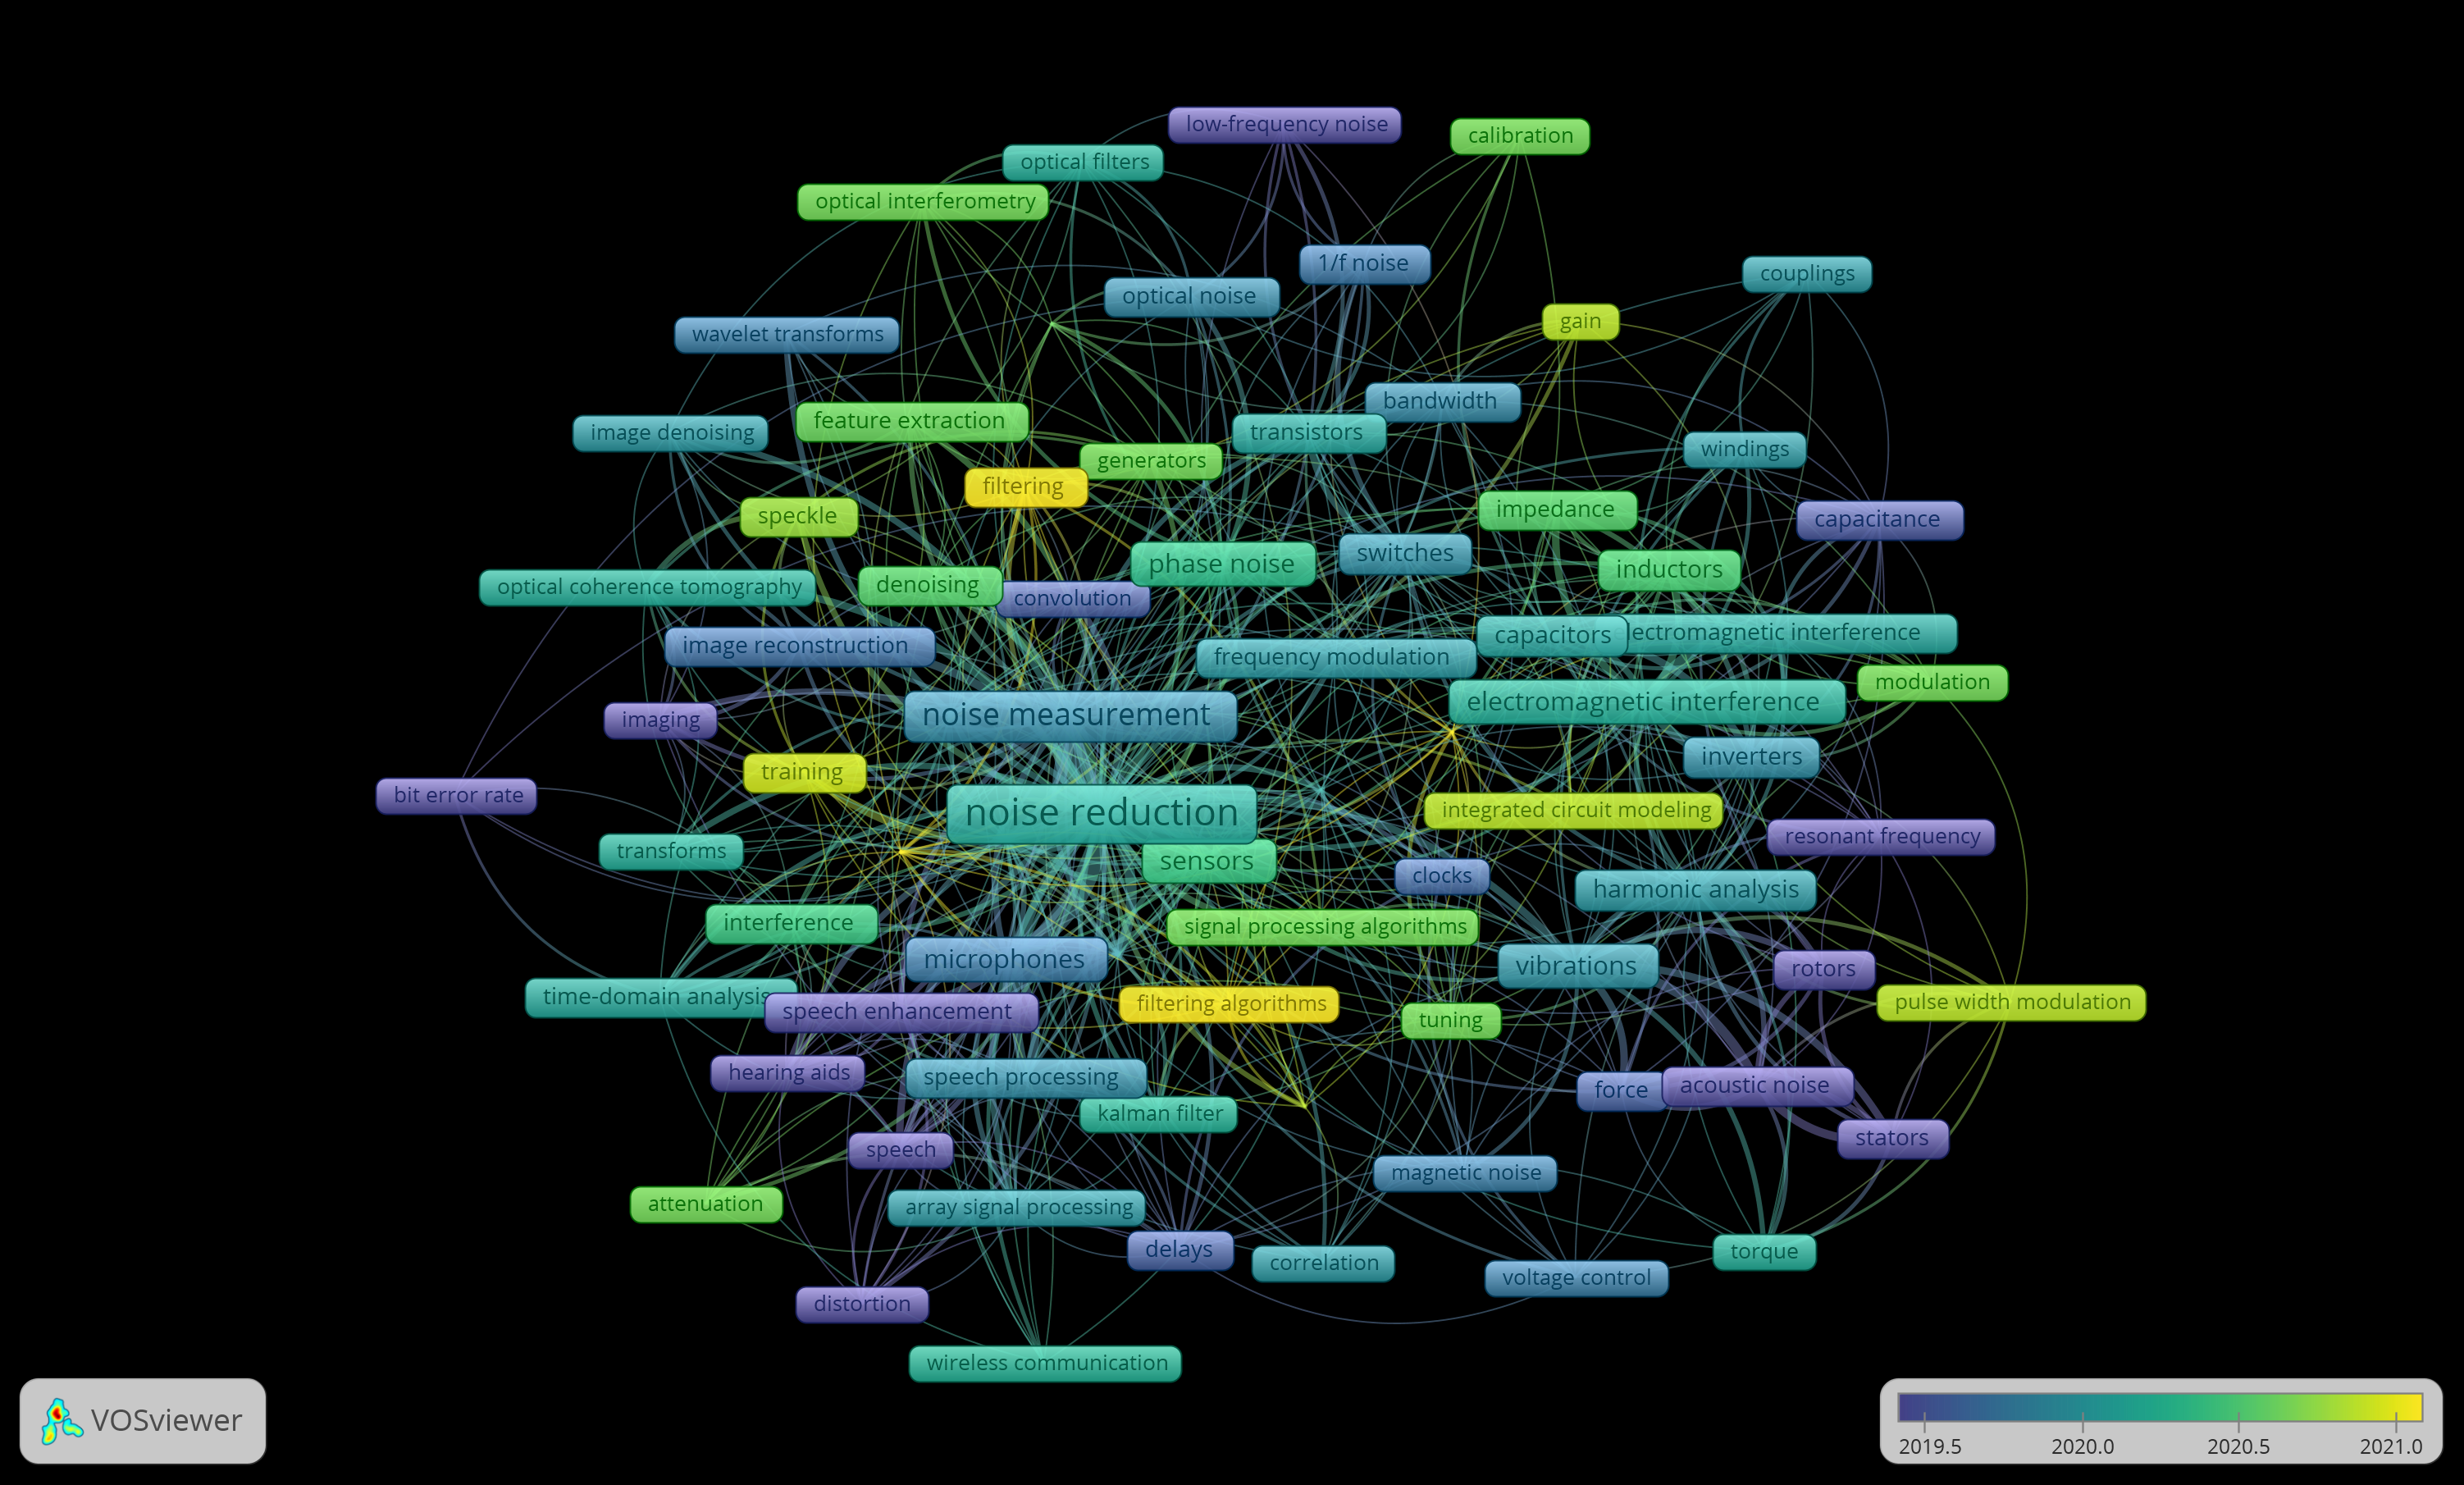
\includegraphics[width=10cm,height=6cm]{../anexos/ris/IEEE/Noise_reduction_and_noise_abatement_andsensor_filtering_algorithm/overlay_visualization.png}
		\end{center}
		\caption{Autor com base no Software VOSViwer}
		\label{figura:network_visualization_with_lines}
	\end{figure}	

\end{frame}

% ----------------- NOVO SLIDE ---------------------- %

\section{Metodologia}

	\begin{frame}{Metodologia}
		\framesubtitle{Materiais}
		\begin{itemize}
			\item ESP32-DevKitC v1 ESP-WROOM-32U;
			\item Cabo USB-Micro USB;
			\item Protoboard 400 pontos;
			\item Sensor de temperatura termistor de 100k.
		\end{itemize}
	\end{frame}

	\begin{frame}{Metodologia}
		\framesubtitle{Descrição do DataSet}
		\begin{itemize}
			\item 1592 valores;
			\item Média de 37.19◦c;
			\item Flutuando entre 1.05◦c e 97.35◦c graus;
			\item 2 minutos.
			\item Tratamento em Python
		\end{itemize}
	\end{frame}

	\begin{frame}{Metodologia}
		\framesubtitle{Descrição do DataSet}
		\begin{figure}[!htb]	
			\begin{center}
				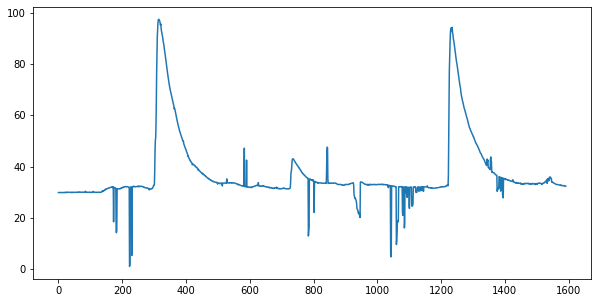
\includegraphics[width=10cm,height=6cm]{../imagens/sensores/bruto.png}
			\end{center}
			\caption{Plotagem gráfica do dataset completo}
			\label{figura:bruto}
		\end{figure}	
	\end{frame}

	\begin{frame}{Metodologia}
		\framesubtitle{Descrição do DataSet}
		\begin{figure}[!htb]	
			\begin{center}
				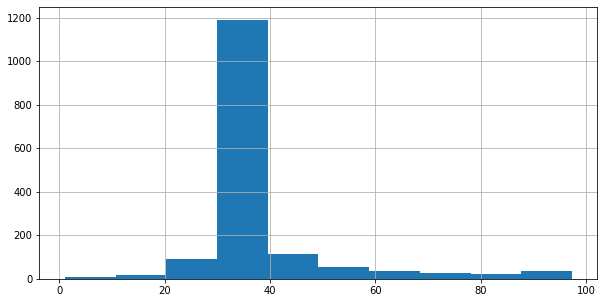
\includegraphics[width=10cm,height=6cm]{../imagens/sensores/hist.png}
			\end{center}
			\caption{histograma do dataset}
			\label{figura:bruto}
		\end{figure}	
	\end{frame}

\section{Resultados}
\begin{frame}[allowframebreaks]
	\scalebox{.6}{                        %new code
	\begin{algorithm}[H]
		\Entrada{Tamanho do vetor de amostras ($TV$), Vetor de amostras ($VA$)}
		\Saida{Valor considerado verdadeiro ($resultado$), Vetor de amostras ($VA$)}
		\Inicio{
			\While{$resultado == SemValor$}{
				$V \leftarrow coletaDadoDoSensor()$; \tcc*[f]{Coleta dado do sensor} \\
	
				% \tcc*[f]{Verifica se o vetor já foi completamente preenchido} \\
				\Se{$tamanho(VA) \geq TV$}{ 
	
					% \tcc*[f]{Retira intervalo de confiança} \\
					$primeiroIntervalo$, $segundoIntervalo \leftarrow intervaloDeConfianca($VA$)$; 
	
					% \tcc*[f]{Verifica se o valor está dentro do intervalo de confiança} \\
					\Se{$V \geq primeiroIntervalo$ \&\& $V \leq segundoIntervalo$}{
						$resultado \leftarrow V$; %\tcc*[f]{Adiciona o valor ao retorno} \\
					}
					
					$VA \rightarrow primeiroElemento$; \tcc*[f]{Remove elemento mais velho} \\
				}
	
				$VA \leftarrow V$; \tcc*[f]{Adiciona valor para dentro do vetor de amostra} \\
			}
	
	
			\tcc*[f]{Retorna valor verdadeiro e vetor com as últimas amostras} \\
			\Retorna $resultado$, $VA$; 
		}
		\caption{Algoritmo para coleta de valor considerado verdadeiro dentro do intervalo de confiança}
		\label{algoritmo:alg1}
	\end{algorithm}
	}

	\scalebox{.5}{                        %new code
	\begin{algorithm}[H]
		\Entrada{Tamanho do vetor de amostras ($TV$), Vetor de amostras ($VA$), Tempo limite de tentativas ($T$)}
		\Saida{Valor considerado verdadeiro ($resultado$), Vetor de amostras ($VA$)}
		\Inicio{
			\While{$resultado == SemValor$}{
	
				$V \leftarrow coletaDadoDoSensor()$; \tcc*[f]{Coleta dado do sensor} \\
	
				\Se{$T \leq 0$}{ 
					$resultado \leftarrow V$;
				}
				$T \rightarrow 1$;  \tcc*[f]{Decrementa tempo} \\
	
				\Se{$tamanho(VA) \geq TV$}{ 
	
					$primeiroIntervalo$, $segundoIntervalo \leftarrow intervaloDeConfianca($VA$)$; 
	
					\Se{$V \geq primeiroIntervalo$ \&\& $V \leq segundoIntervalo$}{
						$resultado \leftarrow V$; 
					}
					
					$VA \rightarrow primeiroElemento$; \tcc*[f]{Remove elemento mais velho} \\
				}
	
				$VA \leftarrow V$; \tcc*[f]{Adiciona valor para dentro do vetor de amostra} \\
			}
	
	
			\tcc*[f]{Retorna valor verdadeiro e vetor com as últimas amostras} \\
			\Retorna $resultado$, $VA$; 
		}
		\caption{Algoritmo que considera o tempo na coleta do sensor}
		\label{algoritmo:alg_com_temp}
	\end{algorithm}
	}

\end{frame}

\begin{frame}{Resultados}
	\framesubtitle{Descrição do DataSet}
	\begin{figure}[!htb]	
		\begin{center}
			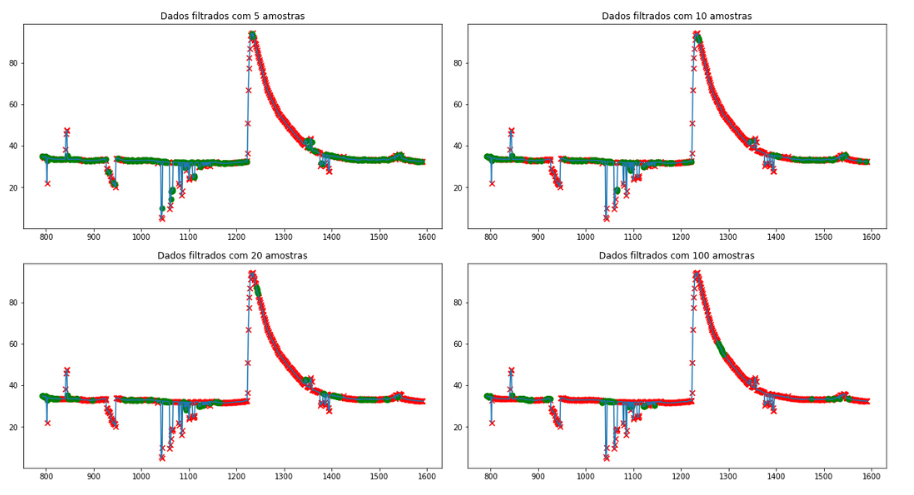
\includegraphics[width=10cm,height=6cm]{../imagens/sensores/graficos_tamanhos_amostras.jpg}
		\end{center}
		\caption{Gráficos mostrando a relação de tamanho da amostra versos quantidade de dados filtrados}
		\label{figura:bruto}
	\end{figure}	
\end{frame}

\begin{frame}{Resultados}
	\framesubtitle{Descrição do DataSet}
	\begin{figure}[!htb]	
		\begin{center}
			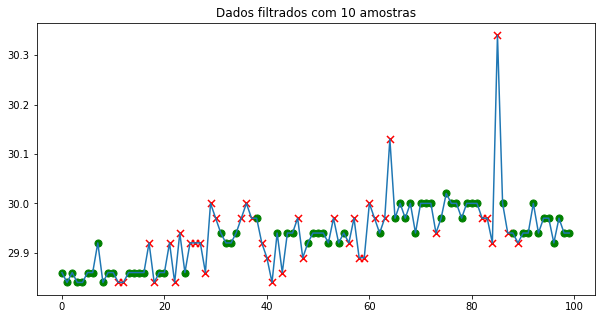
\includegraphics[width=10cm,height=6cm]{../imagens/sensores/filtrado_100_ultimas.png}
		\end{center}
		\caption{Dados de 1530 a 1590}
		\label{figura:bruto}
	\end{figure}	
\end{frame}

\begin{frame}{Resultados}
	\framesubtitle{Descrição do DataSet}
	\begin{figure}[!htb]	
		\begin{center}
			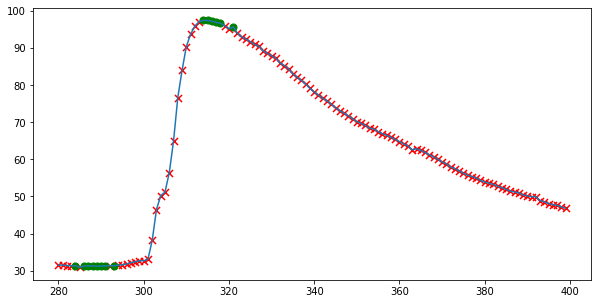
\includegraphics[width=10cm,height=6cm]{../imagens/sensores/indice2.png}
		\end{center}
		\caption{Curva de temperatura no trecho de 280 a 400}
		\label{figura:bruto}
	\end{figure}	
\end{frame}

\begin{frame}{Resultados}
	\framesubtitle{Descrição do DataSet}
	\begin{figure}[!htb]	
		\begin{center}
			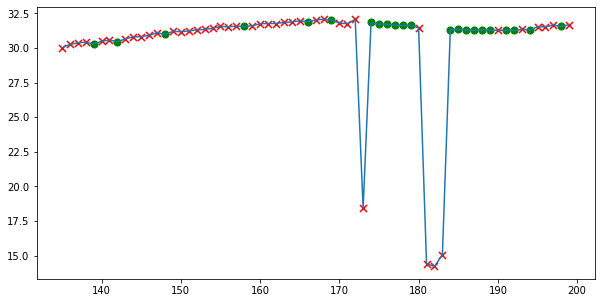
\includegraphics[width=10cm,height=6cm]{../imagens/sensores/indice4.png}
		\end{center}
		\caption{Dataset de 130 a 200}
		\label{figura:bruto}
	\end{figure}	
\end{frame}

\begin{frame}{Resultados}
	\framesubtitle{Descrição do DataSet}
	\begin{figure}[!htb]	
		\begin{center}
			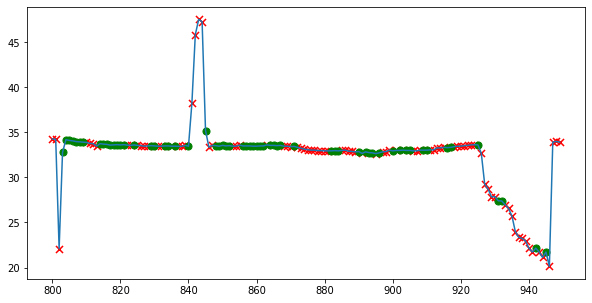
\includegraphics[width=10cm,height=6cm]{../imagens/sensores/indice3.png}
		\end{center}
		\caption{Dados de 800 a 950}
		\label{figura:bruto}
	\end{figure}	
\end{frame}

\section{Conclusões}
\begin{frame}{Conclusões}
	\begin{itemize}
		\item Valores originais dentro de um intervalo de confiança;
        \item Dificuldade em registrar sinais em curvas muito prolongadas e tempo de coleta;
		\item Possibilidade do método ser utilizado em conjunto com outros métodos.
        	
	\end{itemize}
\end{frame}

\begin{frame}{Trabalhos futuros}
	\begin{itemize}
		\item Utilizar o filtro apresentado com outras funções de filtragem.
    	\item Escrever o filtro em uma aplicação real de coleta de dados.
	\end{itemize}
\end{frame}
% ----------------- NOVO SLIDE --------------------------------

\section{Referências}

\begin{frame}[allowframebreaks]{Referências}
	ARAB, H. et al. A hybrid lstm-resnet deep neural network for noise reduction and
	classification of v-band receiver signals. IEEE Access, v. 10, p. 14797–14806, 2022. ISSN
	2169-3536.


	CHIANG, H.-T. et al. Noise reduction in ecg signals using fully convolutional denoising
	autoencoders. IEEE Access, v. 7, p. 60806–60813, 2019.


	DUARTE-SALAZAR, C. A. et al. Speckle noise reduction in ultrasound images for
	improving the metrological evaluation of biomedical applications: An overview. IEEE
	Access, v. 8, p. 15983–15999, 2020. ISSN 2169-3536.


	GOKCESU, K. et al. An adaptive algorithm for online interference cancellation in emg
	sensors. IEEE Sensors Journal, v. 19, n. 1, p. 214–223, Jan 2019. ISSN 1558-1748.
	HENRIQUES, A. Dificuldades na compreensão de intervalos de confiança: um estudo com
	alunos universitários. Actas do XXII Seminário de Investigação em Educação Matemática,
	2011.


	JADAV, G. M. et al. Adaptive filtering and analysis of eeg signals in the time-frequency
	domain based on the local entropy. EURASIP Journal on Advances in Signal Processing,
	SpringerOpen, v. 2020, n. 1, p. 1–18, 2020.


	JEFFERY, S. et al. A pipelined framework for online cleaning of sensor data streams.
	In: 22nd International Conference on Data Engineering (ICDE’06). [S.l.: s.n.], 2006. p.
	140–140. ISSN 2375-026X.
	KALAMBET, Y. et al. Noise filtering: the ultimate solution? Analytics, Citeseer, v. 1,
	n. 1, p. 50–56, 2011.


	KAMATA, H. et al. Mems gyro array employing array signal processing for interference
	and outlier suppression. In: 2020 IEEE International Symposium on Inertial Sensors and
	Systems (INERTIAL). [S.l.: s.n.], 2020. p. 1–4.


	LIU, H. et al. Interference stripe noise reduction of cmos sensor-based digital holographic
	measurement system. IEEE Photonics Journal, v. 13, n. 3, p. 1–18, June 2021. ISSN
	1943-0655.


	NING, Z. et al. Improved mems magnetometer adaptive filter noise reduction and
	compensation method. IEEE Sensors Journal, v. 22, n. 2, p. 1252–1264, Jan 2022. ISSN
	1558-1748.


	PATINO, C. M.; FERREIRA, J. C. Intervalos de confiança: uma ferramenta útil para
	estimar o tamanho do efeito no mundo real. Jornal Brasileiro de Pneumologia, SciELO
	Brasil, v. 41, p. 565–566, 2015.


	RIBEIRO, L. C. Análise de previsão de demanda em uma loja de roupas e acessórios
	infanto juvenil localizada no interior de são paulo. Pontifícia Universidade Católica de
	Goiás, 2020.


	SANTOS, P. B. d. et al. Educação estatística: o conceito de média móvel no ensino
	fundamental na pandemia da covid-19 no brasil. EDUCAÇÃO ESTATÍSTICA: O
	CONCEITO DE MÉDIA MÓVEL NO ENSINO FUNDAMENTAL NA PANDEMIA DA
	COVID-19 NO BRASIL, Editora Científica Digital, v. 3, n. 12, p. 185–204, 2021.


	TAN, Y. L. et al. Sensoclean: Handling noisy and incomplete data in sensor networks
	using modeling. Main, p. 1–18, 2005.
	WAZLAWICK, R. Metodologia de pesquisa para ciência da computação. [S.l.]: Elsevier
	Brasil, 2017. v. 2.


	Zephyr Project™. The Zephyr Project™ strives to deliver the best-in-class RTOS for
	connected resource-constrained devices, built to be secure and safe. 2021. Disponível em:
	<https://zephyrproject.org/>. Acesso em: 02.09.2021.


	ZHOU, Z. et al. Ambient interferences suppressing for in-situ radiated emissions
	measurement based on array signal processing and adaptive noise cancellation. IEEE
	Transactions on Electromagnetic Compatibility, v. 62, n. 4, p. 1055–1067, Aug 2020. ISSN
	1558-187X.


	ZHUANG, Y. et al. A weighted moving average-based approach for cleaning sensor data.
	In: 27th International Conference on Distributed Computing Systems (ICDCS ’07). [S.l.:
	s.n.], 2007. p. 38–38. ISSN 1063-6927.

\end{frame}

% \begin{frame}[allowframebreaks]{Referências}
% 	%\framesubtitle{\TeX, \LaTeX, and Beamer}
% 	\begin{thebibliography}{9}
% 		\providecommand{\abntrefinfo}[3]{}
% 		\providecommand{\abntbstabout}[1]{}
% 		\abntbstabout{v-1.9.6 }
		
% 		\bibitem[Henriques, Ana 2011]{henriques2011dificuldades}
% 		\abntrefinfo{Henriques, Ana}{henriques2011dificuldades}{2011}
% 		{Henriques, Ana
% 		\emph{Dificuldades na compreens{\~a}o de intervalos de confian{\c{c}}a: um estudo com alunos universit{\'a}rios}.
% 		Actas do XXII Semin{\'a}rio de Investiga{\c{c}}{\~a}o em Educa{\c{c}}{\~a}o Matem{\'a}tica, 2011.}
		
% 		\bibitem[AZUMA 2011]{AZUMA2011}
% 		\abntrefinfo{AZUMA}{AZUMA}{2011}
% 		{AZUMA, R.~M. et~al.
% 		\emph{{Otimiza{\c{c}}{\~{a}}o multiobjetivo em problema de estoque e roteamento
% 		  gerenciados pelo fornecedor}}.
% 		1--113~p. Tese (Mestrado) --- Universidade Estadual de Campinas, 2011.}
		
% 		\bibitem[CORRAR, THE{\'{O}}PHILO e BERGMANN 2004]{CORRAR2004}
% 		\abntrefinfo{CORRAR, THE{\'{O}}PHILO e BERGMANN}{CORRAR; THE{\'{O}}PHILO;
% 		  BERGMANN}{2004}
% 		{CORRAR, L.~J. et al. \emph{{Pesquisa operacional para decis{\~{a}}o em
% 		  contabilidade e administra{\c{c}}{\~{a}}o: contabilometria}}. S{\~{a}}o
% 		  Paulo: Atlas, 2004.}
		
% 		\bibitem[CORREIA 2017]{CORREIA2017}
% 		\abntrefinfo{CORREIA}{CORREIA}{2017}
% 		{CORREIA, A. M.~P.
% 		Monografia, \emph{{An{\'{a}}lise de m{\'{e}}todos escalares aplicados a
% 		  problema multiobjetivos}}. [S.l.]: Universidade Estadual do Tocantins, 2017.
% 		  1--63~p.}
		
% 		\bibitem[COUTINHO 2008]{Coutinho2008}
% 		\abntrefinfo{COUTINHO}{COUTINHO}{2008}
% 		{COUTINHO, B.~C.
% 		\emph{{Proposta de Algoritmo H{\'{i}}brido para o Problema de Tarefas em
% 		  Ambientes Distribu{\'{i}}dos Homog{\^{e}}neos}}.
% 		Tese (Mestrado) --- Universidade Federal do Esp{\'{i}}rito Santo, 2008.}
		
% 		\bibitem[COUTINHO e {DE OLIVEIRA} 2009]{COUTINHO2009}
% 		\abntrefinfo{COUTINHO e {DE OLIVEIRA}}{COUTINHO; {DE OLIVEIRA}}{2009}
% 		{COUTINHO, B.~C.; {DE OLIVEIRA}, E.~S. {Fixa{\c{c}}{\~{a}}o de vari{\'{a}}veis
% 		  do modelo matem{\'{a}}tico aplicado na solu{\c{c}}{\~{a}}o do problema de
% 		  escalonamento de tarefas em ambientes distribu{\'{i}}dos homog{\^{e}}neos}.
% 		\emph{SBPO - Simp{\'{o}}sio Brasileiro de Pesquisa Operacional}, 2009.}
		
% 		\bibitem[ETCHEVERRY 2012]{ETCHEVERRY2012}
% 		\abntrefinfo{ETCHEVERRY}{ETCHEVERRY}{2012}
% 		{ETCHEVERRY, G.~V.
% 		\emph{{Programa{\c{c}}{\~{a}}o de tarefas em m{\'{a}}quinas paralelas
% 		  n{\~{a}}o-relacionadas com tempos de setup dependentes da sequ{\^{e}}ncia}}.
% 		1--54~p. Tese (Mestrado) --- Universidade Federal do Rio Grande do Sul, 2012.}
		
% 		\bibitem[HADDAD 2012]{HADDAD2012}
% 		\abntrefinfo{HADDAD}{HADDAD}{2012}
% 		{HADDAD, M.~N. \emph{{Algoritmos heur{\'{i}}sticos h{\'{i}}bridos para o
% 		  problema de sequenciamento em m{\'{a}}quinas paralelas n{\~{a}}o-relacionadas
% 		  com tempos de prepara{\c{c}}{\~{a}}o dependentes da sequ{\^{e}}ncia}}. 2012.}
		
% 		\bibitem[HILLIER e LIEBERMAN 2006]{HILLIER2006}
% 		\abntrefinfo{HILLIER e LIEBERMAN}{HILLIER; LIEBERMAN}{2006}
% 		{HILLIER, F.~S.; LIEBERMAN, G.~J. \emph{{Introdu{\c{c}}ao a Pesquisa
% 		  Operacional}}. 8. ed. S{\~{a}}o Paulo: McGraw-Hill Interamericana do Brasil
% 		  Ltda, 2006.
% 		ISBN 85-86804-68-1.}
		
% 		\bibitem[HILLIER e LIEBERMAN 2013]{HILLIER2013}
% 		\abntrefinfo{HILLIER e LIEBERMAN}{HILLIER; LIEBERMAN}{2013}
% 		{\underline{\ \ \ \ \ \ \ \ }. \emph{{Introdu{\c{c}}{\~{a}}o {\`{a}} pesquisa
% 		  operacional}}. [S.l.: s.n.], 2013.}
		
% 		\bibitem[KAWAMURA 2006]{KAWAMURA2006}
% 		\abntrefinfo{KAWAMURA}{KAWAMURA}{2006}
% 		{KAWAMURA, M.~S.
% 		\emph{{Aplica{\c{c}}{\~{a}}o do m{\'{e}}todo branch-and-bound na
% 		  programa{\c{c}}{\~{a}}o de tarefas em uma {\'{u}}nica m{\'{a}}quina com data
% 		  de entrega comum sob penalidades de adiantamento e atraso.}}
% 		Tese (Tese de Doutorado) --- Universidade de S{\~{a}}o Paulo, 2006.}
		
% 		\bibitem[MARTINS 2017]{MARTINS2017}
% 		\abntrefinfo{MARTINS}{MARTINS}{2017}
% 		{MARTINS, R.~C. \emph{{An{\'{a}}lise de algoritmos evolucion{\'{a}}rios na
% 		  resolu{\c{c}}{\~{a}}o de fun{\c{c}}{\~{o}}es de benchmark irrestritas.}}
% 		  [S.l.]: Universidade Estadual do Tocantins, 2017.}
		
% 		\bibitem[MINEIRO 2007]{MINEIRO2007}
% 		\abntrefinfo{MINEIRO}{MINEIRO}{2007}
% 		{MINEIRO, A.
% 		\emph{{Aplica{\c{c}}{\~{a}}o de programa{\c{c}}{\~{a}}o n{\~{a}}o-linear como
% 		  ferramenta de aux{\'{i}}lio {\`{a}} tomada de decis{\~{a}}o na gest{\~{a}}o
% 		  de um clube de investimento}}.
% 		91~p. Tese (Mestrado) --- UNIFEI, Itajub{\'{a}}, 2007.}
		
% 		\bibitem[M{\"{U}}LLER e DIAS 2002]{MULLER2002}
% 		\abntrefinfo{M{\"{U}}LLER e DIAS}{M{\"{U}}LLER; DIAS}{2002}
% 		{M{\"{U}}LLER, F.~M.; DIAS, O.~B. {Algoritmo para o problema de
% 		  seq{\"{u}}enciamento em m{\'{a}}quinas paralelas n{\~{a}}o-relacionadas}.
% 		\emph{Revista Produ{\c{c}}{\~{a}}o}, v.~12, n.~2, p. 6--17, 2002.
% 		ISSN 0103-6513.}
		
% 		\bibitem[NARI{\~{N}}O, MARTHA e {DE MENEZES} 2014]{NARINO2014}
% 		\abntrefinfo{NARI{\~{N}}O, MARTHA e {DE MENEZES}}{NARI{\~{N}}O; MARTHA; {DE
% 		  MENEZES}}{2014}
% 		{NARI{\~{N}}O, G. A.~R. et al.
% 		\emph{{Otimiza{\c{c}}{\~{a}}o de risers em caten{\'{a}}ria com amortecedores
% 		  hidrodin{\^{a}}micos}}.
% 		18~p. Tese (Mestrado) --- PUC-Rio, 2014.}
		
% 		\bibitem[PACHAMANOVA e FABOZZI 2010]{PACHAMANOVA2010}
% 		\abntrefinfo{PACHAMANOVA e FABOZZI}{PACHAMANOVA; FABOZZI}{2010}
% 		{PACHAMANOVA, D.~A.; FABOZZI, F.~J. \emph{{Simulation and Optimization in
% 		  Finance: Modeling with MATLAB,@ RISK, or VBA}}. [S.l.]: John Wiley {\&} Sons,
% 		  2010. 787~p.
% 		ISBN 9780470371893.}
		
% 		\bibitem[QUEIROZ 2011]{QUEIROZ2011}
% 		\abntrefinfo{QUEIROZ}{QUEIROZ}{2011}
% 		{QUEIROZ, M.~M. de.
% 		\emph{{M{\'{e}}todos heur{\'{i}}sticos aplicados ao problema de
% 		  programa{\c{c}}{\~{a}}o da frota de navios PLVs}}.
% 		Tese (Doutorado) --- Universidade de S{\~{a}}o Paulo, 2011.}
		
% 		\bibitem[REIS, DUQUE e VILLELA 2010]{REIS2010}
% 		\abntrefinfo{REIS, DUQUE e VILLELA}{REIS; DUQUE; VILLELA}{2010}
% 		{REIS, D.~C. et al. {Problema da Aloca{\c{c}}{\~{a}}o de Monitores de Qualidade
% 		  de Energia El{\'{e}}trica em Redes de Transmiss{\~{a}}o}.
% 		\emph{XVIII Congresso Brasileiro de Autom{\'{a}}tica}, p.~1--6, 2010.}
		
% 		\bibitem[ROCHA 2006]{ROCHA2006}
% 		\abntrefinfo{ROCHA}{ROCHA}{2006}
% 		{ROCHA, P.~L.
% 		\emph{{Um problema de sequenciamento em m{\'{a}}quinas paralelas
% 		  n{\~{a}}o-relacionadas com tempos de prepara{\c{c}}{\~{a}}o dependentes de
% 		  m{\'{a}}quina e da sequ{\^{e}}ncia:: modelos e algoritmos exato}}.
% 		1--70~p. Tese (Mestrado) --- Universidade Federal de Minas Gerais, 2006.}
		
% 		\bibitem[SECCHI 2015]{SECCHI2015}
% 		\abntrefinfo{SECCHI}{SECCHI}{2015}
% 		{SECCHI, A.~R. \emph{{COQ-897 - Otimiza{\c{c}}{\~{a}}o de Processos}}. Rio de
% 		  Janeiro: [s.n.], 2015.}
		
% 		\bibitem[SERAFINI, ANZANELLO e KAHMANN 2016]{SERAFINI2016}
% 		\abntrefinfo{SERAFINI, ANZANELLO e KAHMANN}{SERAFINI; ANZANELLO; KAHMANN}{2016}
% 		{SERAFINI, L. et al. {Heur{\'{i}}stica para minimiza{\c{c}}{\~{a}}o do atraso
% 		  total de tarefas baseada em curvas de aprendizado e aspectos
% 		  ergon{\^{o}}micos}.
% 		\emph{Revista Produ{\c{c}}{\~{a}}o Online}, Florian{\'{o}}polis, p. 550--574,
% 		  2016.}
		
% 		\bibitem[SILVA 2008]{SILVA2008}
% 		\abntrefinfo{SILVA}{SILVA}{2008}
% 		{SILVA, V.~V. et~al. {Uma heur{\'{i}}stica h{\'{i}}brida para o problema de
% 		  escalonamento de tarefas peri{\'{o}}dico em m{\'{a}}quinas paralelas}.
% 		\emph{XXVIII Encontro Nacional de Engenharia de Produ{\c{c}}{\~{a}}o}, p.
% 		  1--13, 2008.}
		
% 		\bibitem[XAVIER 2003]{XAVIER2003}
% 		\abntrefinfo{XAVIER}{XAVIER}{2003}
% 		{XAVIER, E.~C. et~al.
% 		\emph{{Algoritmos de aproxima{\c{c}}{\~{a}}o para problemas de escalonamento de
% 		  tarefas em maquinas}}.
% 		1--148~p. Tese (Mestrado) --- Unicamp, 2003.}
		
% 		\bibitem[YUNES 2000]{YUNES2000}
% 		\abntrefinfo{YUNES}{YUNES}{2000}
% 		{YUNES, T.~H. et~al.
% 		\emph{{Problemas de escalonamento no transporte coletivo:
% 		  programa{\c{c}}{\~{a}}o por restri{\c{c}}{\~{o}}es e outras tecnicas}}.
% 		Tese (Mestrado) --- Unicamp, 2000.}
		
% 	\end{thebibliography}
%   \end{frame}
% ----------------- FIM DO DOCUMENTO -----------------------------------------
\end{document}
